
%\textbf{Faculty PI: Kaushik De, Andrew White}
The Intermediate Tile Calorimeter (ITC) was designed to fill the
gaps between the central barrel calorimeter and the extended
barrel calorimeters. Figure~\ref{fig:itc_layout_energy} shows a schematic
view of part of the ATLAS calorimeter, showing the
components of the ITC. For particles which originate at the
nominal interaction point, the ITC extends over approximately $0.8
< |\eta| < 1.6$. The region $0.8 < |\eta| < 0.9$ contains 311 mm
thick steel-scintillator stacks, similar in design to standard
Tile Calorimeter submodules. Between $0.9 < |\eta| < 1.0$, the
stacks are 96 mm in the $z$-direction. The combined $0.8 < |\eta|
< 1.0$ region of the ITC is called the plug. In combination with
the support structure for the scintillators, it is called the ITC
submodule. For the forward region, the active elements of the ITC
consist of scintillator only due to space constraints. The
scintillators between $1.0 < |\eta| < 1.2$ are called the gap
scintillators, while those between $1.2 < |\eta| < 1.6$ are called
cryostat scintillators. The plug and gap scintillator extensions
primarily provide hadronic shower sampling, while the cryostat
scintillators play an important role in sampling electromagnetic
showers. Together, these detectors improve the measurement of
total energy in the intermediate region, thereby improving the jet
and \met\ resolution of ATLAS.

\begin{figure}[htb]
\centering
\subfigure[]{%
      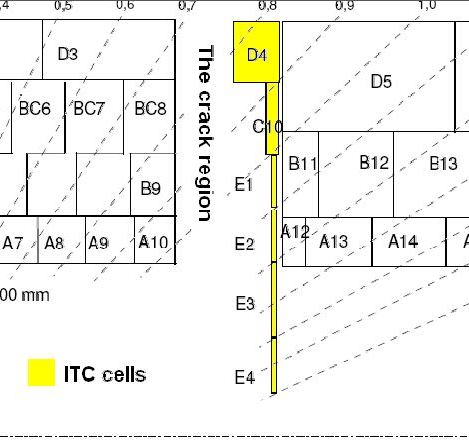
\includegraphics[scale=0.38]{Figures/ITC_region.jpg}
      \label{fig:itc_layout_energy}
           }
\quad
\subfigure[] {%
       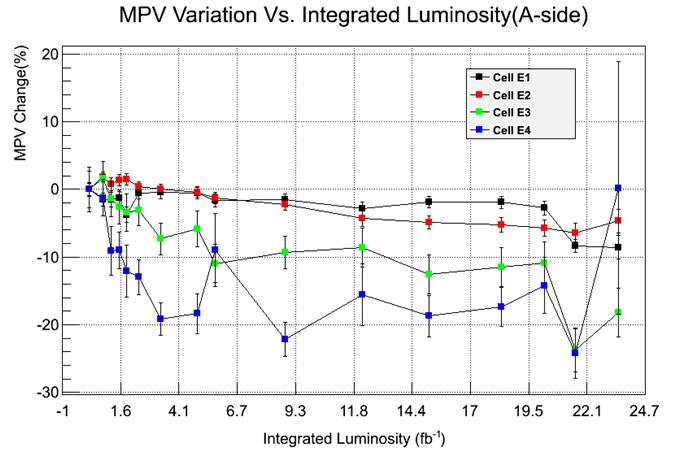
\includegraphics[scale=0.6]{Figures/itc_MPV_vs_Int_Lumi.jpg}
       \label{fig:Change_vs_Lumi}
           }

\caption{Left - Layout of the Intermediate Tile Calorimeter. Right - Average change for ITC E-modules vs. integrated luminosity.}
\end{figure} 

The ITC was proposed by De, who has served as the US ITC project manager (level 2) for the past 15 years. This unique detector was fully designed, constructed and is now maintained by US groups. 
%KD - removed. Not relevant. Can go in White accommplishment. 
% Our group had previously been 
% responsible for the D0 Intercryostat Detector, invented by White, to solve
% the issue of poor jet energy resolution in the gap between the barrel
% and endcap calorimeters. 
All of the ITC submodules and half of the ITC scintillators were
constructed and assembled at UTA, while the remaining parts and assembly were done at Michigan State University (MSU) and Argonne National Laboratory (ANL). Throughout the construction and commissioning phases of ATLAS, De's group had involvement in all aspects of ATLAS hadronic Tile Calorimeter (TileCal): calorimeter module construction, electronics, readout, commissioning and maintenance. White was involved in some early work on ITC mechanical support design, and recently is taking charge of the ITC Phase 2 upgrade. The role of the ITC was highlighted recently when its inclusion in the analysis of a Higgs to
four electron event caused the four electron mass to be moved down by 3 \GeV
which resulted in the event moving into the Higgs signal region.

De's group will continue to play a crucial role in ATLAS hadronic calorimetry. De's postdoc Usai, who is supported 20\% under the base program for ATLAS service work (Usai is supported 45\% through project funds), coordinates UTA  work on TileCal. Usai is located at CERN. He supervises the work of UTA graduate students stationed at CERN that perform service work on TileCal. He works with De's student Darmora to provide regular calibration updates of the ITC using the Cesium (Cs) calibration system. Usai also played a major role in developing the MobiDick4 portable DAQ system, which is being used during LS1 to check and repair Tile eletronics.

Usai's work as TileCal Signal Reconstruction Task Force leader has become increasingly important recently as higher luminosity at the LHC has forced a re-evaluation of the algorithm for hadronic energy measurement. Careful checking of the electronics data and algorithms used are required to cope with the increased pileup of background events. This work will continue to be an important focus, along with error management of TileCal channels, at the start of LHC Run 2 in 2015.

In addition to calibration issues for the ITC, there
is a concern that the scintillator is degrading due to radiation exposure
during data taking. To study this, and decide on a possible strategy to replace 
the scintillator tiles in an ITC upgrade, White with Park and graduate student
Bonde, have been analyzing the energy deposition spectra for individual ITC
tiles across the full range of data taking periods. The energy distribution
for each tile is fitted with a combination of Gaussian (for the noise) and a
convolution of a Gaussian and Landau for the signal part. An average percentage
change (with respect to an early data run) is the calculated for all 64 tiles
in a fixed $ \eta $ interval for each end of the calorimeter. A result for extended 
barrel A is shown in Figure~\ref{fig:Change_vs_Lumi}. Some of the E4 energy 
distributions have been difficult to fit and this leads to the rather unstable
nature of the changes in the figure. We are in the process of refining and optimizing 
the fitting procedure. 

A significant part of the \~{}10\% change for E3 and the \~{}20\% change for E4 is
accounted for by a drop in the photocathode response of the PMTs as they are
illuminated during a run. Detailed results from laser studies of the photocathodes,
combined with the energy distribution fits, show that there is so far about a \~{}5\% change
attributable to the radiation exposure of the scintillator.

Based on the observed changes in the tile signals, it has been decided to replace
a limited number (probably about 6) of the E3 and E4 tiles at each end of the calorimeter.
The replacements are scheduled for Fall 2013 and Spring 2014 as access to the ITC
regions becomes available. In the longer term, we are studying the possible
replacement of all the ITC E1 - E4 tiles with more radiation hard scintillator. 
Figure~\ref{fig:Radiation_dose} shows that, for an integrated luminosity of 100 pb$^-1$,
in Phase-0 the maximum dose for E4 would be 1000 Gy. For the Bicron or ELJEN
scintillator materials this would mean about a 20\% loss in light yield, but
possibly a more serious loss in light transmission through the tiles as seen in Figure~\ref{fig:Transmission_dose}
We are testing several proposed replacement scintillator materials at a proton and gamma
radiation facility at the University of Wittwatersrand since existing data are
rather thin for the dose region of interest for future ITC upgrades. With Michigan State U.
we have completed an MOU for the tile replacement work. The new tiles, fibers, and
connectors will be purchased in 2016, prepared for installation in 2017, and installed
and commissioned in 2018. The funding is anticipated to be provided from non-US Tilecal
institutes, while US (UTA and MSU) will contribute expertise and manpower.


\begin{figure}[htb]
\centering
\subfigure{%
      \includegraphics[scale=0.23]{Figures/R_Z_rad_dose_E3E4_14_TeV.jpg}
      \label{fig:Radiation_dose}
           }
%
%
\quad
\subfigure{%
       \includegraphics[scale=0.35]{Figures/Scintillator_irradiation_transmission.jpg}
       \label{fig:Transmission_dose}
           }

\caption{Left - Radiation doses expected in ITC E3, E4 region. Right - Effect of radiation dose on transmission.}
\end{figure} 

In FY14 we will continue to refine our fits to ITC tile energy distributions to prepare
diagnostic tools to apply to future data, and will develop plans for material selection 
for tile and fiber replacement. In FY15 - FY16 we will work with other tile calorimeter
institutes on the acquisition, preparation, and assembly of tiles, fibers, connectors,
and mechanical items in preparation for installation in LS2 - planned for calendar 2018.
We have been asked by ATLAS Tilecal management to be responsible for monitoring the
performance and quality of data from the ITC using collision and cosmic muons in Run 2.

In order to continue the study of radiation effects on the ITC for the current data, 
to support the investigation of alternative scintillator materials and their
testing, and to plan for the replacement of ITC tiles, the partial support for
a post-doctoral associate is requested by PI White.
% KD - old style - PI: De, White; Postdoc: Usai; Student: Bonde

\fourhead{Tile Calorimeter Operations (PI:Farbin)} \label{sec:af_tile}

%\textbf{Faculty PI: Amir Farbin}
Farbin and his group have retained their connection to TileCal since
2004.  Most recently, Farbin served a deputy run coordinator and
trigger contact in 2010.  His student Heather Brown developed
algorithms for calibrating the special Intermediate TileCal sells as
her 2011 master's thesis. His postdoc Heelan just finished serving as
the TileCal run coordinator and his student Bullock will obtain his
ATLAS qualification on TileCal.

Heelan's tenure as TileCal deputy run coordinator (Jan-Apr) and run
coordinator (May-Aug) has been a 24 hours a day, 7 days a week
commitment that she maintained for 8 consecutive months.  The role
started while the ATLAS detector continued to take collision data,
primarily for heavy ion physics. Since start of the Long Shutdown 1
(LS1) in February, she has been managing a large number of tasks aimed
at improving data quality and data-taking efficiency in Run II. These
include replacing all old LVPS, consolidate the front-end electronics,
fixing all known front-end problems, replacing Minimum Bias Trigger
Scintillators, preparing large D-cells in the extended barrel to help
reduce the muon trigger fake rate in the muon system, and repairing
and improve the leaking cesium garages. As deputy she coordinated the
around the clock shifts of the number teams working on the detector,
provided all instructions, documentation, and training, and running or
attending various operations meetings. 

As run coordinator she compiled and maintained the list of problems
with the front-end electronics, coordinated all TileCal personnel and
their daily activities based on scaffolding accesses, data quality
results, initial status of the drawer, and actions for repair.  She
managed all calibrations and served as the link between the data
quality team and various hardware maintenance teams. She helped
consolidate more than 100 drawers, almost completing all drawers with
initial problems that have been repaired.

% She also became the primary expert
% on the Tile detector verification system (DVS) package, which tests
% the read out and timing trigger control for one drawer by sending
% signals to the front-end electronics and reading back the response.

% She helped consolidate more than 100 drawers, almost completing all
% drawers with initial problems that have been repaired. Near the end of
% her term as Run Coordinator, the Tile teams gained access to the
% extended barrels, which have fewer initial problems, but were going to
% undergo modifications. She helped develop the work plan for this
% portion of the detector.


%% - To compile a list of all initial problems for each of the 256 drawers:
%% https://docs.google.com/spreadsheet/ccc?key=0AnWucdRMgbe8dDcyakZZaW5VNGlRTXZpb1hJRXdxWWc#gid=0
%% and convert this into a more human readable format for the maintenance teams to use while working underground:
%% http://atlas.web.cern.ch/Atlas/SUB_DETECTORS/TILE/DP_files/TileCalMaintenanceKnownIssues.pdf
%% This has been an ongoing project

%% - Coordinate a team of people: two maintenance coordinators, two operations coordinators, 2-3 teams of two people working underground, data quality leader and validator, DCS experts

%% - To coordinate daily meetings with the team to coordinate activities for the day/week, based on scaffolding accesses, data quality results, initial status of the drawer, actions for repair, etc.

%% - Coordinate a weekly Tile operations meeting: knowledge of relevant activities, request reports, follow-up on outstanding action items 

%% - Facilitate communication between the ATLAS Operations Management/Technical Coordination and the Tile calorimeter group through weekly meetings

%% - I coordinated (contacting experts, compiling lists, finalizing actions) problems related to cases where bits get stuck in the on or off position, and problems relating to (the still mostly not understood) cases where the digitizer will jump in time by 25 ns (a problem difficult to detect during data taking and can severally affect the reconstruction, a problem that will be almost impossible to detect when protons will collide every 25 ns).  

%% - Be the expert of the Tile detector verification system (DVS)
%%   package, which tests the read out and timing trigger control for one
%%   drawer by sending signals to the front-end electronics and reading
%%   back the response. The previous expert of the system left the
%%   experiment and it was charged to the run coordinators to run the
%%   tests and maintain the system. These tests are performed before
%%   every drawer is opened, and after it is consolidated and closed. It
%%   is the first test to use the complete data acquisition chain used by
%%   ATLAS and used to quickly identify any problems.

% - Be the link between data quality and the maintenance hardware team by:
%   -- requesting and helping in changes to the calibration qualification tests more appropriate for the maintenance period and problems being found/solved 
%   -- give quick feedback to the maintenance hardware team working the ATLAS cavern results from the calibrations
%   -- attending several weekly meetings 

% - 2-3 times per week take full calibrations, and special calibrations as requested. Note laser calibrations are only taken when there are no people working in the pit.

% - Work with the LUCID team to help setup use of the Tile laser calibration system for LUCID in Run II.

% - Be one of the main people responsible for updating and overseeing the progress of the consolidation process; this was tracked using both a web interface and elogs:
% https://tilecal.web.cern.ch/tilecal/TileLS1Status/pub/
% https://pcata007.cern.ch/elog/Maintenance/

% - Created and maintained the Tile LS1 Operations wiki:
% https://twiki.cern.ch/twiki/bin/viewauth/Atlas/TileLS1Operation

% - Write reports after a majority of a partition is completed to evaluate if the problems have been solved, if new ones have appeared, and agree on the course of action with the team. As RC, I worked with the team to consolidate more than 100 drawers, almost completing all drawers in the two long barrels which had many different initial problems that have since been repaired. 

% - Near the end of my term as RC the teams gained access to the extended barrels, which have fewer initial problems, but were going to undergo modifications. After much iteration, it was decided to modify the 3-in-1 card integrator gains for the E-cells (gap/crack scintillators) that tend to see large amounts of energy and were approaching saturation during Run I. For similar reasons the HV passive divider is being replaced by an HV active divider on two E-cell PMTs. There is currently work to modify calibration tests were necessary, like the integrator gains test, to account for the changes in these PMTs. 


% These responsibilities required me to be on-call 24 hours a day, 7 days a week, for 8 consecutive months. 

